\documentclass[10pt]{article}
\usepackage{amsmath}
\usepackage{amssymb}
\usepackage{amsthm}
\usepackage{geometry}
\usepackage{tikz}
\geometry{margin=1in}

\newtheorem{definition}{Definition}
\newtheorem{lemma}{Lemma}
\newtheorem{theorem}{Theorem}
\newtheorem{example}{Example}
\newtheorem{note}{Note}

\title{Probability and Statistics Notes\\Complete Collection}
\author{John Linke}
\date{September 18, 2024}

\begin{document}

% Include each section from separate files
% To use this master file, save each artifact as its own .tex file
% and uncomment the appropriate \input commands below:

% If you have separate files, use:
\section{Sample Spaces}

\begin{definition}
An experiment is any process that can be repeated with a well-defined set of outcomes. Example: roll a die, toss a coin.
\end{definition}

\textbf{Sets:} discrete/finite, discrete/infinite, continuous

\begin{definition}
A sample space is the set of all possible outcomes of an experiment. Example: $S = \{1, 2, 3, 4, 5, 6\}$, $S = \{H, T\}$
\end{definition}

\begin{definition}
The union of $A$ and $B$, $A \cup B$, is all elements in $A$ or $B$.
\end{definition}

\begin{definition}
The intersection of $A$ and $B$, $A \cap B$, is all elements in both $A$ and $B$.
\end{definition}

\begin{definition}
$A$ and $B$ are mutually exclusive (disjoint) if $A \cap B = \emptyset$.
\end{definition}

\begin{definition}
The complement of $A$, $A^c$, is the set of elements not in $A$: $S - A$.
\end{definition}

\section{Probability}

\begin{definition}
The function $P$ is a probability function if it satisfies:
\begin{enumerate}
\item $P(A) \in [0, 1]$ for all $A \subseteq S$
\item $P(S) = 1$
\item If $A$ and $B$ are disjoint, then $P(A \cup B) = P(A) + P(B)$
\item If $A_1, A_2, \ldots$ are disjoint, then $P\left(\bigcup_{i=1}^{\infty} A_i\right) = \sum_{i=1}^{\infty} P(A_i)$
\end{enumerate}
\end{definition}

\begin{lemma}
$P(A^c) = 1 - P(A)$
\end{lemma}

\textbf{Proof:} $A \cup A^c = S$, $A \cap A^c = \emptyset$, so $P(S) = P(A \cup A^c) = P(A) + P(A^c) = 1$. Therefore, $P(A^c) = 1 - P(A)$.

\subsection{Fair Dice Example}
If we roll a fair die, $P(i) = \frac{1}{6}$ for $i = 1, 2, \ldots, 6$.

$P(\{1, 2\} \cup \{3, 4\} \cup \{5, 6\}) = P(\{1\}) + P(\{2\}) + \cdots + P(\{6\}) = 6 \cdot P(\{1\}) \Rightarrow P(\{1\}) = \frac{1}{6}$

Note: If all elements in $S$ are equally likely, $P(A) = \frac{\text{\# in } A}{\text{\# in } S}$

\subsection{Card Example}
Roll a fair dice, find $P(\text{sum} = 5)$.

\begin{center}
\begin{tabular}{c|cccc}
 & $A$ & $B$ & Total \\
\hline
 & 1 & 4 & 5 \\
 & 2 & 3 & 5 \\
 & 3 & 2 & 5 \\
 & 4 & 1 & 5
\end{tabular}
\end{center}

There are 26 people, find $P(\text{at least 2 same birthday})$.

$1 - P(\text{0 different})$

\begin{lemma}[Addition Rule]
$P(A \cup B) = P(A) + P(B) - P(A \cap B)$
\end{lemma}

If disjoint: $P(A \cup B) = P(A) + P(B) - 0 = P(A) + P(B)$

Proof: $P(A \cup B^c) + P(A \cap B^c) + P(B \cap A^c) = P(A \cup B)$

\textbf{Prove:} If $A \subseteq B$, then $P(A) \leq P(B)$

If $A \subseteq B$, $B^c \cap A = \emptyset$

$B = A \cup (A^c \cap B)$ (disjoint union), so $P(B) = P(A) + P(A^c \cap B)$

Because $P(\cdot)$ is non-negative, $P(B) \geq P(A)$

\section{Counting}

\subsection{Example 2.8}
Given $A, B, C$:
\begin{enumerate}
\item[a)] none occur: $A^c \cap B^c \cap C^c$ (only $A$ occurs: $A \cap B^c \cap C^c$)
\item[b)] all three occur: $A \cap B \cap C$ (exactly one occurs: $(A \cap B^c \cap C^c) \cup (A^c \cap B \cap C^c) \cup (A^c \cap B^c \cap C)$)
\item[c)] at least one occurs: $A \cup B \cup C$ ($(A^c \cap B \cap C) \cup (A \cap B^c \cap C)$)
\end{enumerate}

$P(A) = 0.3$, $P(B) = 0.7$, $P(A \cap B) = 0.1$, WANTED

$P(A \cup B) = 0.3 + 0.7 - P(A \cap B) = 0.9 - 0.5 = 0.4$

Blue/green/red

$P(A \cup B) = 0.5 + 0.7 = P(A \cap B) = 0.9$

$P(A \cap B) = 0.3$

\begin{center}
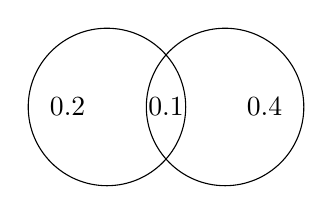
\begin{tikzpicture}
\draw (0,0) circle (1cm);
\draw (1.5,0) circle (1cm);
\node at (-0.5,0) {0.2};
\node at (2,0) {0.4};
\node at (0.75,0) {0.1};
\end{tikzpicture}
\end{center}

\subsection{Counting Example}
Choose a card at random: $P(A) = \frac{3}{7}$, $P(A \cap \text{red}) = \frac{15}{70} = \frac{3}{14}$, $P(A \cup \text{red}) = \frac{4}{7}$

Choose two at random without replacement (conditional probability): if the first card has an $A$, find $P(\text{second} = A) = \frac{2}{69}$, $P(\{2^{\text{nd}} = A\} \mid \{1^{\text{st}} = A\}) = \frac{1}{51} = \frac{1}{17}$

One card: $P(\text{red} \mid A) = \frac{15}{30} = 0.5$

$P(\text{red} \mid A) = \frac{P(\text{red} \cap A)}{P(A)} = \frac{3/7}{1} = \frac{3}{7}$

\section{Conditional Probability}

\begin{definition}
$P(A \mid B) = \frac{P(A \cap B)}{P(B)}$
\end{definition}

Choose two without replacement: $P(\text{both blue}) = P(\{1^{\text{st}} \text{ blue} \cap 2^{\text{nd}} \text{ blue}\}) = P(\text{blue})P(2^{\text{nd}} \text{ blue} \mid 1^{\text{st}} \text{ blue})$

$= \frac{14}{70} \cdot \frac{13}{69} = \frac{182}{4830} = \frac{14}{70} = \frac{1}{5}$

Choose 5 without replacement: $P(\text{at least one is blue}) = 1 - P(\text{no blue}) = 1 - \frac{56 \cdot 55 \cdots}{70 \cdot 69 \cdots}$

Example: Two buckets - 11 blue/1 green, 2 blue/3 green. Choose one from bucket one and move to bucket 2, choose 1 from bucket 2:

$P(1^{\text{st}} \text{ blue} \cap 2^{\text{nd}} \text{ blue}) = \text{WORK}$

$P(1^{\text{st}} \text{ green} \cap 2^{\text{nd}} \text{ blue}) = \frac{1}{4}$

$P(2^{\text{nd}} \text{ blue}) = \frac{6}{12}$

\subsection{Total Probability - Given Events}
Total probability: Given $A_1, A_2, \ldots, A_n$ with $A_i \cap A_j = \emptyset$ ($i \neq j$) and $\bigcup A_i = S$,

then $P(B) = \sum_{i=1}^n P(B \cap A_i) = \sum_{i=1}^n P(A_i)P(B \mid A_i)$



\section{Conditional Probability (continued)}

Find $P(1^{\text{st}} \text{ blue} \mid 2^{\text{nd}} \text{ blue}) = \frac{P(1^{\text{st}} \text{ blue} \cap 2^{\text{nd}} \text{ blue})}{P(2^{\text{nd}} \text{ blue})} = \frac{4/4}{5/12} = 0.6$

See setup for total probability.

\begin{theorem}[Bayes' Theorem]
\[P(A \mid B) = \frac{P(B \mid A)P(A)}{P(B)} = \frac{P(B \cap A)P(A)}{\sum_{\text{all } k} P(B \mid A_k)P(A_k)}\]
\end{theorem}

\subsection{Medical Test Example}

A test is 95\% accurate: $P(\{+\} \mid \text{disease}) = 0.95$, $P(\{-\} \mid \text{not disease}) = 0.95$

If $P(\text{disease}) = 0.01$, find $P(\text{test} +)$:

\begin{align*}
0.01 \cdot 0.95 &= (0.01)(0.95) + (1.00)(0.05) = 0.059
\end{align*}

$P(\text{disease} \mid +) = \frac{P(\text{is } + \text{ } \cap)}{P(+)} = \frac{(0.01)(0.95)}{0.059} = 0.16$

Roll a die until you get a 6:

$P(\{3\}) + P(\{4\}) + P(\{5\}) = \left(\frac{5}{6}\right)^2 \left(\frac{1}{6}\right) + \left(\frac{5}{6}\right)^3 \left(\frac{1}{6}\right) + \left(\frac{5}{6}\right)^4 \left(\frac{1}{6}\right)$

Geometric sequence: $a + ar + ar^2 + \cdots = \frac{a}{1-r}$ if $|r| < 1$

$a = \frac{1}{6}$, $r = \frac{5}{6}$, so $\left(\frac{5}{6}\right)^2 \left(\frac{1}{6}\right) = \frac{a \cdot r^2}{1 - r} = \frac{(1/6)(5/6)^2}{1/6} = \frac{25}{36}$

Question 2 if $r \geq 1$

$P$ if $A \subseteq B$, then $P(A) \leq P(B)$

\section{Homework}

\subsection{Roll 2 dice}
Find $P(\text{sum} = 6)$: $S' = \{2, 3, 4, \ldots, 12\}$, $S_Y = \{0, 1, 2, \ldots\}$

Roll 2 dice: Find $P(\text{exactly 4 green})$

$n = 10$, $k = 4$, $p = \frac{10}{50} = 0.2$, $P(4 \text{ green}) = \binom{10}{4}(0.2)^4(0.8)^6$

Binomial pdf $(n, p, k)$: $n \binom{n}{k} = \frac{n!}{k!(n-k)!}$

Choose 5 without replacement:

\subsection{Discrete Random Variables}

\begin{example}
Roll 2 dice: $X = $ sum of two rolls, $Y = \#$ of 6s

$S_X = \{2, 3, 4, \ldots, 12\}$, $S_Y = \{0, 1, 2\}$

Example: Roll 1 dice, let $X = (1^{\text{st}} \text{ roll})$, $Y = \#$ of $\{$

$S_X = \{2, 3, 4, \ldots, 12\}$, $S_Y = \{0, 1, 2, 3\}$
\end{example}

\begin{theorem}
A random variable $X$ is a function from a sample set to the real numbers (with an associated probability distribution).
\end{theorem}

\textbf{Example:} Roll two dice: $X = $ sum of two rolls, $Y = \#$ of $\{$

$S_X = \{2, 3, 4, \ldots, 12\}$, $S_Y = \{0, 1, 2, 3\}$

\begin{theorem}
Associated with a random variable is a probability density function (pdf) which gives the probability of all elements.
\end{theorem}

\begin{theorem}
The cumulative distribution function (cdf) for $X$ is: $F_X(x) = P(X \leq x)$
\end{theorem}

\section{Binomial Distribution}

\begin{definition}
$P(X = k) = \binom{n}{k} p^k (1-p)^{n-k}$, $k = 0, 1, 2, \ldots, n$

where $n = \#$ of trials, $k = \#$ of successes, $p = P(\text{success in one trial})$, $\binom{n}{k} = $ number of ways choosing $k$ out of $n$
\end{definition}

\begin{example}
50 red, 40 red, 10 green

Choose 10 with replacement: Find $P(\text{exactly 4 green})$

$n = 10$, $k = 4$, $p = \frac{10}{50} = 0.2$, $P(4 \text{ green}) = \binom{10}{4}(0.2)^4(0.8)^6$
\end{example}

\textbf{Binompdf} $(n, p, k)$: $n \binom{n}{k} = \frac{n!}{k!(n-k)!}$

Choose 5 without

\section{Discrete Random Variables}

\begin{example}
Roll 2 dice, find $P(\text{sum} = 5)$

Choose 10 with replacement: Find $P(\text{exactly 4 green})$

$n = 10$, $k = 4$, $p = \frac{10}{50}$, $p = 0.2$

$P(4 \text{ green}) = \binom{10}{4}(0.2)^4(0.8)^6$
\end{example}

\section{Continuous Random Variables}

\begin{example}
Choose a number at random from the interval $[0, 100]$ in $\mathbb{R}$:

$P(X \leq 50) = 0.5$, $P(X \leq 10) = \frac{1}{10}$, $P(X \leq 1) = \frac{1}{100}$, $P(X = 0) = 0$

$P(X \leq V_1) = \int_0^{V_1} p_{2-x} dx = \frac{x^2}{2} \Big|_0^{V_1} = \frac{V_1}{4}$
\end{example}

\begin{example}
$P_X(x) = 2x$, $0 \leq x \leq 1$

$P(X \leq V_1) = P(X \leq V_1) = \int_0^{V_1}$
\end{example}

\begin{definition}
For $P_X(x)$ to be a pdf, we need: $f_X(x) \geq 0$, $\int_{-\infty}^{\infty} f_X(x) dx = 1$
\end{definition}

Find the cdf $F_X(x) = P(X \leq x) = \int_{-\infty}^x 2x dx = x^2 \Big|_0^x = x^2$ for $0 \leq x \leq 1$

\begin{example}
$f_X(x) = 2e^{-2x}$, $x \geq 0$

$P(X \geq 1) \int_1^{\infty} 2e^{-2x} dx = -e^{-2x} \Big|_1^{\infty} = 0 + e^{-2}$
\end{example}

$f_X(x) = cx^2 e^{x^3}$, $x \geq 0$

Find $c$ so this is a pdf:

$1 = \int_0^{\infty} cx^2 e^{x^3} dx = c\left(-\frac{1}{3} e^{-x^3}\right) \Big|_0^{\infty} = \frac{c}{3} (0 - (-1)) = \frac{c}{3}$

$c = 3$

$P_X(x) = 3x^2 e^{-x^3}$

Find $c$ for pdf: $1 = \int_0^{\infty} c x e^{-2x} dx$

$u = -\frac{1}{2} e^{-2x}$, $dv = x dx$

$dv = 1$, $dv = e^{-x}$

$c\left[-\frac{1}{2} x e^{-2x} - \frac{1}{4} e^{-2x}\right] \Big|_0^{\infty} = c \cdot \frac{1}{4} = 1$, $c = 4$

$f_X(x) = 2x$, $0 \leq x \leq 1$

If $y = 2x + 1$, find $P_Y(y)$

Go through: $F_Y(y) = P(Y \leq y) = P(2x + 1 \leq y) = P\left(x \leq \frac{y-1}{2}\right)$

$= \int_0^{\frac{y-1}{2}} 2x dx = x^2 \Big|_0^{\frac{y-1}{2}} = \left(\frac{y-1}{2}\right)^2 = \frac{(y-1)^2}{4}$, $1 \leq y \leq 3$

$f_Y(y) = \frac{d}{dy}(y-1)^2 = \frac{(y-1)}{2}$ pdf

\section{Expected Value}

\begin{example}
We have: 3, 2.5, 4, 3.5, 2, 5.5. Mean: $\frac{7.5}{20} = 3.75$

$2\left(\frac{3}{20}\right) + 3\left(\frac{8}{20}\right) + 5\left(\frac{2}{20}\right) = \sum_{i} n_i P(n_i)$
\end{example}

\begin{definition}
The expected value of a random variable $X$ is:

\[E(X) = \begin{cases}
\sum_{x \in S} x \cdot P(X = x) & \text{discrete} \\
\int_{-\infty}^{\infty} x \cdot f_X(x) dx & \text{continuous}
\end{cases}\]
\end{definition}

\begin{example}
$P(X = x) = \frac{1}{10}$, $x = 1, 2, 3, 4$

$E(X) = \frac{1}{10}[1 + 2 + 3 + 4] = 3$

$P(X = 1) = \frac{1}{10}$
\end{example}

Roll a die until the first 6, with $\#$ of rolls: Find $E(X)$

$P(X = 1) = \frac{1}{6}$, $P(X = 2) = \left(\frac{5}{6}\right)\left(\frac{1}{6}\right)$, $P(X = k) = \left(\frac{5}{6}\right)^{k-1} \left(\frac{1}{6}\right)$, $k = 1, 2, \ldots$

$E(X) = \sum_{k=1}^{\infty} k \cdot \left(\frac{5}{6}\right)^{k-1} \left(\frac{1}{6}\right)$

$\sum ar^k = \frac{a}{1-r}$, $a + 2ar + 3ar^2 + \cdots = \frac{a}{(1-r)^2}$, $E(X) = \frac{1/6}{(1-5/6)^2} = 6$

Binomial: $P(X = k) = \binom{n}{k} p^k (1-p)^{n-k}$, $k = 0, 1, \ldots, n$

$E(X) = \sum_{k=0}^n k \binom{n}{k} p^k (1-p)^{n-k} = np$

\subsection{Continuous Example}

$f_X(x) = 2x$, $0 \leq x \leq 1$

$E(X) = \int_0^1 x(2x^2) dx = \frac{2}{3}$

$f_X(x) = 2e^{-2x}$, $x \geq 0$

$E(X) = \int_0^{\infty} x \cdot 2e^{-2x} dx \Rightarrow \hat{\lambda} = \frac{1}{2}$

Toss a coin until the first $T$, if it's on 1st win 1

$1 \cdot P(T \text{ on } 1^{\text{st}}) + 2 \cdot P(T \text{ on } 2^{\text{nd}}) + \cdots = 2^n E(W_n) = 2\left(\frac{1}{2}\right) + 4\left(\frac{1}{4}\right) + \cdots + 2^n \left(\frac{1}{2^n}\right) = \sum_{n=1}^{\infty} 1 = \infty$

$f_X(x) = \frac{1}{2}$, $x \geq 1$

Show this is a pdf:

$1 = \int_1^{\infty} \frac{c}{x^2} dx = -\frac{c}{x} \Big|_1^{\infty} = 0 + 1 = 1 \checkmark$

$E(X) = \int_1^{\infty} x \left(\frac{1}{x^2}\right) dx = \ln(x) \Big|_1^{\infty} = \infty$

\section{Median}

\begin{definition}
The median $m$ is the number so that $P(X \leq m^*) \geq 0.5$ and $P(X \geq m^*) \geq 0.5$.
\end{definition}

\begin{example}
$P_X(x) = 3x^2$, $0 \leq x \leq 1$

$0.5 = \int_0^{m^*} 3x^2 dx$, so $0.5 = x^3 \Big|_0^{m^*} = (m^*)^3$, thus $m^* = \sqrt[3]{0.5}$
\end{example}

\textbf{Notation:} $E(X) = \mu$, $\bar{X} = \frac{1}{n} \sum_{i=1}^n X_i$ (population mean vs sample mean)

\begin{note}
$E(g(x)) = \sum g(x) P(X = x)$ or $\int_{-\infty}^{\infty} g(x) P_X(x) dx$
\end{note}

\begin{example}
$x = [-1, 1, 3]$

\[E(X) = -0.3 + 0.4 + 0.9 = 1\]

$E(\cos(x)) = \cos(-1)(0.3) + \cos(1)(0.2) + \cos(3)(0.3)$

$E(X) = \int_0^1 3x^3 dx$, $E(x^2) = \int_0^1 x^2(3x^2) dx$
\end{example}

\section{Variance}

\begin{definition}
\[\text{Var}(X) = E[(X - \mu)^2] = \sigma^2 \qquad 1, 2, 5 \Rightarrow \sigma^2 = 2 \qquad \text{Var} = 4\]
\end{definition}

\begin{theorem}
$E[(X - \mu)^2] = \text{Var}(X) = E(X^2) - \mu^2$
\end{theorem}

\begin{note}
$E(aX + b) = aE(X) + b$
\end{note}

\section{Variance Examples}

\begin{example}[Finite discrete dist.]
$x = 1, 2, 3, 4$, $E(X) = \frac{1}{4}(1 + 2 + 3 + 4) = 2.5$

$\text{Var}(X) = \frac{1}{4}[(1 - 2.5)^2 + (2 - 2.5)^2 + (3 - 2.5)^2 + (4 - 2.5)^2] = 1.25$
\end{example}

\begin{example}[Roll die]
$E(X) = \frac{1}{6}(1 + 2 + 3 + 4 + 5 + 6) = 3.5$

$E(X^2) = \frac{1}{6}(1 + 4 + 9 + 16 + 25 + 36) = \frac{91}{6}$

$\text{Var}(X) = \frac{91}{6} - (3.5)^2 = \frac{35}{12}$
\end{example}

\begin{example}[Binomial]
$E(X) = np$, $\text{Var}(X) = np(1 - p)$

Roll 600, $k \neq$ of 6's: $E(X) = 100$, $\text{Var}(X) = 600 \cdot \frac{1}{6} \cdot \frac{5}{6}$
\end{example}

\section{Further Properties of Mean and Variance}

\begin{theorem}[Lemma]
$E(aX + bY) = aE(X) + bE(Y)$
\end{theorem}

\textbf{Useless:} $\sigma = S(+)+EY + \sqrt{VAR}$

\begin{definition}
$\bar{X} = \frac{1}{n} \sum X_i$ where $X_i$ are from a list with $E(X_i) = \mu$

$E(\bar{X}) = \frac{1}{n} \sum E(X_i) = \mu$
\end{definition}

\begin{note}
$\text{Var}(\bar{X}) = E[(\bar{X} - \mu)^2] = E\left[\left(\frac{1}{n} \sum X_i - \mu\right)^2\right] = E\left[X^2\right] - \mu^2$
\end{note}

\begin{note}
If $X$ and $Y$ are independent, $\text{Var}(X) + \text{Var}(Y)$
\end{note}

$\text{Var}(aX + bY)$ if $X$ and $Y$ are independent: $a^2 \text{Var}(X) + b^2 \text{Var}(Y)$

$\text{Var}(X_1 + \cdots + X_n) = \text{Var}(X_1) + \cdots + \text{Var}(X_n)$ if $X$ and $Y$ are independent

$\text{Var}(\bar{X}) = \sigma^2$ where $\sigma^2 = \text{Var}(X_i) = \frac{\sigma^2}{n}$

\textbf{Notation (if points equally likely):} $\sigma^2 = \frac{1}{n} \sum (X_i - \mu)^2$ = population variance

$s^2 = \frac{1}{n-1} \sum (X_i - \bar{X})^2$ = sample variance

\begin{center}
\begin{tabular}{c|cccccc}
$Y$ & 1 & 2 & 3 & 4 & 5 & 6 \\
\hline
$X$ & 1 & 1 & 1 & 1 & 1 & 1 \\
1 & $\times$ & & & & & \\
2 & $\times$ & $\times$ & & & & \\
3 & $\times$ & $\times$ & $\times$ & & & \\
4 & $\times$ & $\times$ & $\times$ & $\times$ & & \\
5 & & & & & $\times$ & \\
6 & & & & & & $\times$
\end{tabular}
\end{center}

PMF with respect to $Y$

\section{The k-th Moment}

\begin{definition}
The k-th moment of $X$ is $E(X^k)$
\end{definition}

\textbf{Notation (if points equally likely):} $\sigma^2 = \frac{1}{n} \sum (X_i - \mu)^2$ = population variance = standard

$s^2 = \frac{1}{n-1} \sum (X_i - \bar{X})^2$ = sample var

\section{Joint Densities}

\begin{example}
$f_{X,Y}(x,y) = \frac{2}{3} xy$, $0 \leq x \leq 1$, $0 \leq y \leq 2$, $x + y > 1$

Find $E(XY) = \int \int (xy) \left[\frac{2}{3} xy\right] dy dx = \frac{2}{3} \int_0^1 \int_{1-x}^2 x^2 y^2 dy dx$

Find $F(X) = \int_0^2 \frac{2}{3} xy dy = \frac{2}{3} xy \Big|_{y=0}^{2} = \frac{2}{3} x(2) - \frac{2}{3} x(0) = \frac{4}{3}x$, $0 \leq x \leq 1$

Expected $f(x)$: $P(Y > X) = 1 - P(Y \leq X) = 1 - \int_0^1 \int_0^x \frac{2}{3} xy dy dx$

$y = \begin{bmatrix} y_1 \\ \vdots \\ y_n \end{bmatrix}$, $z = \begin{bmatrix} z_1 \\ \vdots \\ z_n \end{bmatrix}$

Find $E(XY) = \sum \sum (xy) P(X,Y) = (.5)(2)(.5) + 1.5$

$E(Y) = 1(.3) + 1(.6) + 2(.1) = .5$

Find $E(XY) = (.1)(.1) + (.2) + 2(.2) + 2(.3) + 2(.2) + 2(.3) = .6$
\end{example}

\begin{definition}
The covariance is the $\text{Cov}(X,Y) = E[(X - \mu_X)(Y - \mu_Y)] = E(XY) - E(X)E(Y)$
\end{definition}

Are the sets $\{x=13\}$ and $\{y=13\}$ independent? $P(\{x=13\} \cap \{y=13\}) = P(\{x=13\})P(\{y=13\})$

$P(\{x=x\})$ 

\begin{theorem}
The random variables $X$ and $Y$ are independent if $P(X \in A \cap Y \in B) = P(X \in A)P(Y \in B)$ for all sets $A \in S_X$, $B \in S_Y$
\end{theorem}

If $X$ and $Y$ are independent, $E(XY) = E(X)E(Y) \Rightarrow \text{Cov}(X,Y) = 0$

\textbf{Lemma:} The continuous random variables $X$ and $Y$ are independent if $f_{XY}(x,y) = g(x)h(y)$ where $g(x) = k f_X(x)$ and $h(y) = \ell f_Y(y)$ for all $x \in S_X$, $y \in S_Y$

\begin{example}
$f_{XY}(x,y) = \frac{1}{33} xy$, $0 \leq x \leq 1$, $0 \leq y \leq 2$, $x + y > 1$

Are $X$ and $Y$ independent? NO - need 5 to be rectangle
\end{example}

\begin{example}
$f_{XY}(x,y) = d(x \cdot y)$, $0 \leq x \leq 2$, $0 \leq y \leq 5$

$f_{XY}(x,y) = \frac{1}{(x+y)} p \neq h(x)g(y)$ NO
\end{example}

\begin{example}
$f_{XY}(x,y) = e^{-(x+y)}$, $x \geq 0$, $y \geq 0$

$= e^{-x} \cdot e^{-y} = g(x) h(y)$ YES
\end{example}

\begin{example}
If $\text{Var } f_X(x) = 4x^3$, $0 \leq x \leq 1$, $f_Y(y) = 3y^2$, $0 \leq y \leq 1$

Find $P(Y > X)$: If $Y$ and $Y$ are independent

$f_{XY}(x,y) = 4x^3(3y^2) \Rightarrow$

$\int_0^1 \int_x^1 (2x^3y^2) dy dx = \int_0^1 4x^3 y^3 \Big|_x^1 dx$

$\ldots$
\end{example}

\section{Further Properties of Mean and Variance}

\begin{lemma}
$E(aX + bY) = aE(X) + bE(Y)$
\end{lemma}

\begin{definition}
$\bar{X} = \frac{1}{n} \sum X_i$ where $X_i$ are from a list with $E(X_i) = \mu$

$E(\bar{X}) = \frac{1}{n} \sum E(X_i) = \mu$

$\text{Note: } \text{Var}(\bar{X}) = E[(\bar{X}-\mu)^2] = E[(X_i - \mu)]^2 = E[X^2] - \mu^2$
\end{definition}

\begin{note}
If $X$ and $Y$ are independent, $\text{Var}(X+Y) = \text{Var}(X) + \text{Var}(Y)$
\end{note}

$\text{Var}(aX + bY)$ if $X$ and $Y$ are independent $= a^2 \text{Var}(X) + b^2 \text{Var}(Y)$

$\text{Var}(\bar{X})$ for $X$ and $Y$ independent: $\sigma^2 = \text{Var}(X_i) = \frac{1}{n^2}[\sigma^2 + \cdots + \sigma^2] = \frac{\sigma^2}{n}$

$\text{Var}(N) = 100\sigma^2(X) - 36\text{Var}(Y) - 110\sigma^2(X) + 36\text{Var}(Y)$ if $X$ and $Y$ are $ind$

\begin{definition}
The correlation coefficient is: $\rho = \frac{\text{Cov}(X,Y)}{\sigma_X \sigma_Y}$, $-1 \leq \rho \leq 1$
\end{definition}

PPP:
\begin{enumerate}
\item $-1 \leq \rho \leq 1$
\item $\rho = \pm 1 \Leftrightarrow y = a + bx$
\item $\rho = 0$ no linear association
\item $\rho$ gives the percent of the variation in $y$ due to the change in $x$
\end{enumerate}

\begin{example}[20]
$X \sim \text{Binom}(n, p_x)$, $Y \sim \text{Binom}(m, p_y)$, $U = X + Y$

Find $E(U)$, $\text{Var}(U)$

$E(X) = np_x$, $E(Y) = mp_y$, $\text{Var}(X) = np_x(1 - p_x)$, $\text{Var}(Y) = mp_y(1 - p_y)$

$E(U) = 4E(X) + 6E(Y) = 4np_x + 6mp_y$

$\text{Var}(N) = 10\sigma^2(X) - 36\text{Var}(Y) = 110p_x(1 - p_x) + 36mp_y(1 - p_y)$ if $X$ and $Y$ are $ind$
\end{example}

\section{The Poisson Distribution}

\begin{definition}
The Poisson distribution is: $P(X = k) = \frac{e^{-\lambda} \lambda^k}{k!}$ for $k \in \mathbb{N}$ (or $k = 0, 1, \ldots$)

$E(X) = \lambda = \text{Var}(X)$
\end{definition}

This usually gives the number of occurrences in a time interval. Something is Poisson if:
\begin{enumerate}
\item The occurrences in $\Delta t$ happen simultaneously
\item For a short enough time frame, there are 0 or 1 occurrences
\item Occurrences are independent
\item The rate of occurrences is constant (only matters well if a $\Delta t$-age unit 2 small)
\end{enumerate}

\begin{example}
A TV has 6 million pixels, where the probability that one is defective is $\frac{1}{2}$ mill. $\lambda = $ mean = 5 A mill/2 mill = 2.5

$P(3 \text{ are defective}) \approx e^{-2.5} \frac{(2.5)^3}{3!} = P(\text{Poisson} p(\lambda = 2.5, k)) = 0.2136$
\end{example}

Find $P(X \geq 3)$: WORK = Poisson $p(\lambda = 2.5, k)$

\begin{example}
The number of people who walk into a store is Poisson with a mean of $\frac{50}{1 \text{ hour}}$. Find $P(\text{at least in one hour with Poisson} p(\lambda = 2.5, k))$ or $P(3 \text{ in } 10 \text{ mins})$

$\lambda = 3$, Poisson $p(\lambda = 5, k) = 0.104$
\end{example}

\textbf{Note:} If the number of occurrences is Poisson, then the time between occurrences is exponential: $P(X = k) = \lambda e^{-\lambda k}$ (ECN $\Rightarrow X$)

\begin{example}
The mean is 492 for two hours: $\lambda = 492$ (for 2 hours)

Find $\lambda$ (in 2 min): $\lambda = \frac{492}{60} \approx 8.0333$, $\lambda^{492}/60 = 8.0333$

Therefore Poisson $p(\lambda = 492/60, k) = 0.029$ or $P(E3; \text{ in } 2 \text{ min}) = $ Poisson $p(\lambda = 492/60, k) = 0.014$
\end{example}

Find $P(E3; \text{ in } 2 \text{ min}) = $ Poisson $p(\lambda = 492/60, k)$

\begin{example}
20000 People play, if $P(\text{win}) = \frac{1}{5000}$. Find $P(2>$ People win)

$\lambda = \frac{20000}{5000} = 4$, $1 - P(X \leq 3) = 1 - \text{Poisson} \text{CDF}(4, 2) = \bar{7}(2)$
\end{example}

\section{The Normal/Gaussian Distribution}

\begin{definition}
Normal/Gaussian distribution: $f_X(x) = \frac{1}{\sigma\sqrt{2\pi}} e^{-\frac{1}{2}\left(\frac{x-\mu}{\sigma}\right)^2}$, $-\infty < x < \infty$, $-\infty < \mu < \infty$, $\sigma > 0$

Standard: $f_Z(z) = \frac{1}{\sqrt{2\pi}} e^{-\frac{z^2}{2}}$, human
\end{definition}

\begin{example}
Find $P(2 \leq (1.2)) = $ Normal $\text{CDF}(2, 100000, 1.2) \cap \mu = 0$ $\Rightarrow P = 0.8849$

\textbf{Lemma:} If $X$ is Normal with $\mu = 100$, $\sigma = 10$

Find $P(2 \leq (1.2))$ If we take a sample of 100 $P(\bar{X} > 52)$ = Normal $\text{CDF}(52, 100000, 50)$

Find a so: $P(\mu = k \leq \mu)$ $\Rightarrow$ inv Normal $\text{CDF}(.75, 100, 10, \text{center})$
\end{example}

HW 3

Bernoulli: $P(X = 1) = p$, $P(X = 0) = 1 - p$

\begin{enumerate}
\item[a)] Find $E(X)$ and $\text{Var}(X)$

$E(X) = \sum x P(X = x)$ and $\text{Var}(X)$

b) Let $Y = X_1 + X_2 + \cdots + X_n$ when $X_i = \text{Bernoulli}$ with $P(X_i = 1) = p$ and

$E(Y) \cdot \sum x P(X = x)$

$\text{Var}(Y) = \text{Var}(X_1 + \cdots) = np(1 - p)$

$\text{Var}(Y) = \text{Var}(2X_i) \Rightarrow \text{Var}(\bar{X}_i)^2$
\end{enumerate}

\section{Central Limit Theorem}

Given a sample $X_1, X_2, X_3, \ldots X_n$ all from the same population taken independently, then $\bar{X} = \frac{1}{n} \sum X_i$ and the sum $\sum X_i$ are normal

No outliers or strong skewed normal converges under sample $E(\frac{\bar{X} - \mu}{\sigma/\sqrt{n}})$ $\Rightarrow$ so $sd(\bar{X}) = \frac{\sigma}{\sqrt{n}}$, $\text{Var}(\bar{X}) = n\sigma^2$

For $X$ we know $\mu = 50$, $\sigma = 8$

Find $P(\bar{X} > 52) = ?$ If we take a sample of 100 $P(\bar{X} > 52) = $ Normal $\text{CDF}(52, 10000, 50, 30)$

Find $P(X > 52) = ?$ Find a $P(\mu \leq k \leq \mu)$ $\Rightarrow$ $a$ with $P(X \geq 52) = $ Normal $\text{CDF}(52, 10000, 50, 30) = 0.0062$

Find a so that $P(\mu \leq k \leq \mu)$: inv Normal $(1.75, 100, 10, \text{center})$

\begin{example}
$X$ is normal with $\mu = 12$, $\sigma = 42$

Find $P(X \leq 150) = $ Normal $\text{CDF}(10000, 130, 12, 41) = 0.0655$

With a sample of 400: Find $P(10 \leq \bar{X} \leq 1(2)) = $ Normal $\text{CDF}(112, 110, 112, 41/\sqrt{400})$
\end{example}

\begin{example}
Roll a dice 600 times, estimate $P(90 \leq \# \text{ of } 6 \text{'s} \leq 115)$: Mean = $np = 106$

variance $= np(1 - p) = \frac{500}{6} \approx 71.27$

continuity correction: $P(\bar{X} < 70) \Rightarrow P(\bar{X} \leq 70.5)$ $\Rightarrow$

$P(10 \leq k \leq 115) = P(90.52 k \leq 115) = $ Normal $\text{CDF}(115, 90.5, 115.5, 70.5, 100.5)$

$k < 100 \Rightarrow X \leq 100.5$, $X \geq 100 \Rightarrow X \geq 99.5$
\end{example}

\end{document}